% -*- TeX:de -*-
\NeedsTeXFormat{LaTeX2e}
\documentclass[12pt,a4paper]{article}
\usepackage[german]{babel} % german text
\usepackage[DIV12]{typearea} % size of printable area
\usepackage[T1]{fontenc} % font encoding
%\usepackage[latin1]{inputenc} % most likely on Windows
\usepackage[utf8]{inputenc} % probably on Linux
\usepackage{multicol}

% PLOTTING
\usepackage{pgfplots} 
\usepackage{pgfplotstable}
\usepackage{url}
\usepackage{graphicx} % to include images
\usepackage{tikz}
\usepackage{subfigure} % for creating subfigures
\usepackage{amsmath} % a bunch of symbols
\usepackage{amssymb} % even more symbols
\usepackage{booktabs} % pretty tables
\usepackage{makecell} % multi row table heading

% a floating environment for circuits
\usepackage{float}
\usepackage{caption}

%\newfloat{circuit}{tbph}{circuits}
%\floatname{circuit}{Schaltplan}

% a floating environment for diagrams
%\newfloat{diagram}{tbph}{diagrams}
%\floatname{diagram}{Diagramm}

\selectlanguage{german} % use german

\begin{document}

%%%%%%% DECKBLATT %%%%%%%
\thispagestyle{empty}
			\begin{center}
			\Large{Fakultät für Physik}\\
			\end{center}
\begin{verbatim}


\end{verbatim}
							%Eintrag des Wintersemesters
			\begin{center}
			\textbf{\LARGE WS 2013/14}
			\end{center}
\begin{verbatim}


\end{verbatim}
			\begin{center}
			\textbf{\LARGE{Physikalisches Praktikum\\ für das Bachelorstudium}}
			\end{center}
\begin{verbatim}




\end{verbatim}

			\begin{center}
			\textbf{\LARGE{PROTOKOLL}}
			\end{center}
			
\begin{verbatim}

\end{verbatim}

			\begin{flushleft}
			\textbf{\Large{Experiment (Nr., Titel):}}\\
							%Experiment Nr. und Titel statt den Punkten eintragen
			\LARGE{PW11 Wechselstrom II}	
			\end{flushleft}

\begin{verbatim}

\end{verbatim}	
							%Eintragen des Abgabedatums, oder des Erstelldatums des Protokolls
			\begin{flushleft}
			\textbf{\Large{Datum:}} \Large{9.1.2014}
			\end{flushleft}
			
\begin{verbatim}
\end{verbatim}
							%Namen der Protokollschreiber
		\begin{flushleft}
			\textbf{\Large{Namen:}} \Large{Patrick Braun, Johannes Kurz}
			\end{flushleft}

\begin{verbatim}


\end{verbatim}
							%Kurstag und Gruppennummer, zb. Fr/5
			\begin{flushleft}
			\textbf{\Large{Kurstag/Gruppe:}} \Large{DO/2}
			\end{flushleft}

\begin{verbatim}

\end{verbatim}
							%Name des Betreuers, das Praktikum betreute.
			\begin{flushleft}
			\LARGE{\textbf{Betreuer:}}	\Large{Clemens Nagel}	
			\end{flushleft}

%%%%%%% DECKBLATT ENDE %%%%%%%
\pagebreak
\setlength{\columnsep}{20pt}
\begin{multicols}{2}

%%%%%%%%%%%%%%%%%%%%%%%%%%%%%%%%%%%%%%%%%%%%%%%%

%\begin{figure}[H]
%	\centering
%	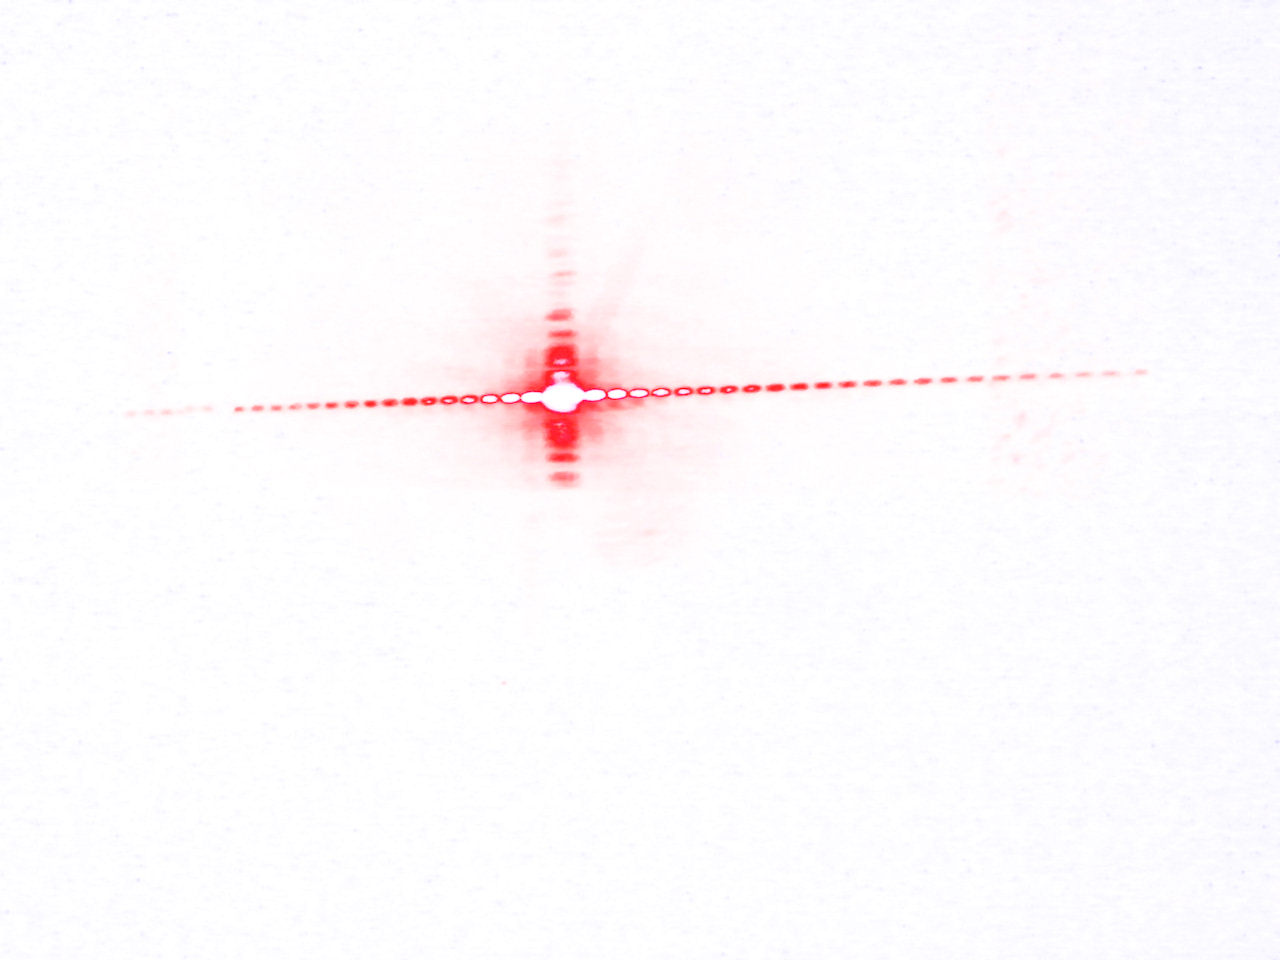
\includegraphics[scale=0.35]{./figure/beugung.png}
%	\caption{Beugungsmuster Einzelspalt (echtes Foto; schwarz durch weiß ersetzt)}
%	\label{fig:beugungsmuster}
%\end{figure}


%\begin{figure}[H]
%	\centering
%	\pgfplotstabletypeset[
%			columns={abstand, n},
%			col sep=&,
%			columns/abstand/.style={precision=2, zerofill, column name=\makecell{$Abstand$\\$(\pm 0.05)[mm]$} }, 
%			columns/n/.style={column name=\makecell{$n$\\$(Ordnung)$}, precision=0},
%			every head row/.style={before row=\hline,after row=\hline\hline},
%			every last row/.style={after row=\hline},
%			every first column/.style={column type/.add={|}{} },
%			every last column/.style={column type/.add={}{|} }
%			]{
%			abstand & n
%			12.9 & 1
%			24.45 & 2
%			37.40 & 3
%			49.35& 4
%			62.45 & 5
%			74.45 & 6
%			87.45 & 7
%			100.25 & 8
%			
%			}
%	\caption{Messwerte Einzelspalt}
%	\label{tab:werte_einzelspalt}
%\end{figure}
%


\section{Theorie}
\subsection{Wechselstrom und Widerstände}
PW11 beschäftigt sich mit Wechselspannungen und-strömen und deren Messung mit dem Oszilloskop.\\
Deren Höhe wechselt, im Gegensatz zu Gleichspannungen und -strömen mit der Zeit, und das in allen betrachteten Anwendungen periodisch. Es kommen also zu Größe und Polarität im Gleichstrom auch Eigenschaften wie Periodendauer $T$, Frequenz $f$ dazu ($f = \frac{1}{T}$ mit der Dimension $[s^{-1}]$ bzw. $Hertz$ (Hz)).\\
\\
In diesem Praktikumsbeispiel werden, wie auch in der öffentlichen Stromversorgung, ausschließlich sinusförmig wechselnde Ströme und Spannungen verwendet, deren Größenverlauf eben einer Sinusfunktion, mit der Zeit im Argument, gleicht.\\
$$U(t)=U_0\cdot sin(\omega t + \varphi_U)$$
$$I(t)=I_0\cdot sin(\omega t + \varphi_I)$$
$U_0$ und $I_0$ sind dabei die Amplituden (also die größte Auslenkung) beider Größen, und $\omega$ die Kreisfrequenz der Schwingung ($\omega = 2 \pi f$).\\
Im Argument des Sinus steht also jeweils ein Winkel, der sich mit der Zeit ändert:
$$\varphi (t) = \omega t$$
Dazu kommen noch die Winkel $\varphi_U$ und $\varphi_I $ bei $t=0$, die sog. Phasenkonstanten. Diese beschreiben einen Versatz des zeitlichen Verlaufs zwischen Spannung und Strom in einem System ($\Delta \varphi = \varphi_u - \varphi_I$).\\
\\
Dieser mathematische Formalismus legt einen Übergang in die komplexen Zahlen nahe, zu einer Beschreibung der Schwingungen als komplexe Exponentialfunktion:
$$\hat{U} = U_0e^{i \omega t + \varphi_U}$$
$$\hat{I} = I_0e^{i \omega t + \varphi_I}$$
wobei die tatsächlichen Spannungen und Ströme zu jeder Zeit dem Realteil entsprechen.\\
Abgesehen von rechentechnischen Vorteilen, bringt diese Darstellung vor allem, dass das Ohm'sche Gesetz und die Kirchhoff'schen Regeln in der komplexen Schreibweise gleich anzuwenden sind, wie in Gleichstrom-Systemen. (Für die reelle Darstellung gilt dies nicht!)\\
\\
In PW11 werden 3 Grundtypen von Widerständen untersucht:\\
Ohm'sche ($R$), kapazitive ($X_C$) und induktive ($X_L$) Widerstände.\\
Im Komplexen lassen sich diese als Impedanz $Z$ nach dem Ohmschen Gesetz berechnen:
$$Z=\frac{\hat{U}}{\hat{I}}=\frac{U_0}{I_0}\cdot e^{i(\varphi_U - \varphi_I)}=\frac{U_0}{I_0}\cdot e^{i \Delta \varphi}$$
Dabei erzeugen Ohm'sche Widerstände keine Phasenunterschiede zwischen Spannung und Strom: $Z_R = R$\\
Kapazitive Widerstände (Kondensatoren) lassen den Strom um $\frac{\pi}{2}$ oder $90^\circ$ der Spannung vorauseilen: $Z_C=-\frac{i}{\omega C}=-i X_C$
Induktive Widerstände (Spulen) erzeugen eine Phasenverschiebung, die den Strom um  $\frac{\pi}{2}$ verschoben, der Spannung hinterherlaufen lässt:$Z_L=i \omega L = i X_L$\\
Die reellen Widerstände sind einfach die  Beträge der komplexen Impedanzen. Phasendifferenzen wirken sich daher nicht auf den reellen Widerstand aus.

\subsection{Aufgaben zur Serienschaltung verschiedener Widerstände}
4 der 6 Aufgabenstellungen drehen sich um die verschiedenen Widerstandstypen in Serienschaltung mit einem bekannten Ohm'schen Widerstand.\\
In Serie geschaltet addieren sich Widerstände auf, wobei bei komplexen Widerständen zu beachten ist, dass der Gesamtwiderstand der Betrag einer komplexen Zahl ist:
$$Z_{ges}=R_0 + iX \Rightarrow |Z_{ges}|=\sqrt{R_0^2+X^2}$$
Es werden in diesen AUfgaben nur Spannungen gemessen. Da die Kirchhoffschen Regeln und das Ohm'sche Gesetz gelten, lässt sich durch die Spannung am bekannten Widerstand der Strom berechnen, der widerum in der gesamten Schaltung gleich ist:
$$\frac{U_{R_0}}{R_0}=I_0=\frac{U_{ges}}{|Z_{ges}|}=\frac{U_{ges}}{\sqrt{R_0^2+X^2}}$$
Daraus kann also der unbekannte Widerstand $X$ berechnet werden.\\
Wie beim Übergang zwischen kartesischer und polarer Darstellung in der komplexen Ebene kann also auch der Phasenverschiebungswinkel, bei bekannten Widerständen berechnet werden durch
$$tan{\Delta \varphi}=\frac{Im(Z_{ges}}{Re(Z_{ges})}=\frac{X}{R_0}$$

\subsection{Einfache elektronische Filter}
Zuletzt soll noch ein Frequenzfilter aufgebaut und untersucht werden.\\
In dieser einfachen Schaltung macht man sich die Frequenzabhängigkeit des Widerstandes eines Kondensators zu Nutze und dass Spannungen an Widerständen, die in Serie geschaltet sind, in derem Verhältnis geteilt werden:
$$\frac{U_1}{R_1}=\frac{U_2}{R_2} \Rightarrow \frac{U_1}{U_2}=\frac{R_1}{R_2} $$
$$Z_C=-\frac{i}{\omega C}=-i X_C$$
An eine Serienschaltung (RC-Glied) aus einem Ohm'schen Widerstand $R$ und einem Kondensator $C$ wird also eine Eingangsspannung $\hat{U_e}$ gelegt und an einem der beiden Bauelemente die Ausgangsspannung $\hat{U_a}$ abgegriffen. Je nach Frequenz von $\hat{U_e}$ wird also $\hat{U_a}$ kleiner oder praktisch gleich der Eingangsspannung. Man sagt, hohe (oder tiefe) Frequenzen werden "durchgelassen" (high-pass/low-pass filter).\\
Die Übertragungsfunktion $A(\omega)$ beschreibt, frequenzabhängig, das Verhältnis von Input und Output.
$$A(\omega)=|A(\omega)|e^{i\Delta \varphi}=\frac{U_a}{U_e}e^{i\Delta \varphi}=\frac{\hat{U_a}}{\hat{U_e}}$$
, wobei $\Delta \varphi$ hier die Phasenverschiebung zwischen Eingangs- und Ausgangsspannung ist.\\
\\
Der Betrag von $A(\omega)$ wird üblicherweise in Dezibel (dB) angegeben, einer logarithmischen Einheit:
$$|A(\omega)| / dB = 20 log{\frac{U_a}{U_e}}$$
Weiters wird die Grenzfrequenz $f_g$ definiert, als die Frequenz, an der die Ausgangsspannung auf das Niveau der Effektivspannung der Eingangsspannung, also $U_{e0}/\sqrt{2}$ abgesunken ist, also auf -3dB. Die Grenzfrequenz kann auch berechnet werden durch
$$f_g=\frac{\omega_g}{2 \pi}= \frac{1}{2 \pi RC}$$

\section{Aufbau und Methoden}

Alle Versuche in PW11 werden auf einem Steckbrett aufgebaut, die zu vermessenden Bauteile sind in mit festen Steckern in den entsprechenden Abständen verbunden.\\
Als Signalquelle dient ein Funktionsgenerator HAMEG HM8040-3, der hier sinusförmige Schwingungen ausgibt.\\
Gemessen wird mit einem Tekronix TPS 2012B Oszilloskop und, in Aufgabe 1, ein Digitalvoltmeter Fluke 175.\\
Sowohl das Oszilloskop (DSO) als auch der Funktionsgenerator sind über Koaxialkabel mit dem Steckbrett verbunden. Diese Kabel bestehen aus 2 Leitungen, wobei der Innenleiter das Signal führt und der Außenleiter $an$ $Masse$ liegt. Es ist in allen Schaltungen daher darauf zu achten, dass die Polung korrekt ist. Wird ein signalführender Leiter direkt mit Masse verbunden, liegt ein Kurzschluss vor.\\


%Tekronix TPS 2012B Oszi\\
%Fluke 175\\
%HAMEG HM8040-3 Stromquelle\\



\subsection{Aufgabe 1}

%SCHALTBILD

In dieser Aufgabe wird die Spannung an einem bekannten Ohm'schen Widerstand ($R_0 = 2.15 k\Omega$) sowohl mit dem DVM als auch dem DSO bei verschiedenen Frequenzen gemessen.\\
Das DVM misst dabei die Effektivspannung $U_{eff}$, mit dem DSO wird die Amplitude $U_0$ gemessen. Dazu muss das DSO so eingestellt werden, dass die Spannungskurve am Bildschirm ruhend dargestellt werden kann. Anschließend kann der Unterschied zwischen 2 Spannungsspitzen $U_{PP}$ gemessen werden, dessen Hälfte die Amplitude ist.\\
Die Messung wird für verschiedene Frequenzen, beginnend mit 100Hz, etwa in 500er Schritten durchgeführt, und der Quotient $U_{eff}/U_0$ gegen die Frequenz aufgetragen.\\
Damit soll überprüft werden, dass das DVM bei höheren Frequenzen ungenauer misst, also der Quotient von einer Gerade abweicht, und ab welchem Frequenzbereich das der Fall ist.



\subsection{Aufgabe 2, 3 und 4}
%SCHALTBILD
In allen 3 Aufgaben, werden der bekannte Widerstand $R_0$ und ein zweiter unbekannter ($R_x$ der Ohm'sche, $X_C$ der kapazitive und $X_L$ der induktive Widerstand) in Serie geschaltet.\\
Mit den beiden Kanälen des DSO werden die Gesamtspannung $U_ges$ und die Spannung $U_0$ am $R_0$ gemessen. Würden die Spannungen an beiden Widerständen gemessen werden, müssten eine signalführende Leitung und eine Masseleitung verbunden werden, was zu einem Kurzschluss führen würde.\\
Der unbekannte Widerstand kann jeweils berechnet werden und die Phasenverschiebung $\Delta \varphi$ ermittelt werden, in dem der Laufzeitunterschied zwischen Spannung und Strom mit dem Cursertool des DSO gemessen werden. (Spannung und Strom sind phasengleich am Funktionsgenerator. Daher ist die Differenz der Phasen der beiden Spannungen gleich der Phasendifferenz zwischen Spannung und Strom, die vom unbekannten Widerstand erzeugt wird.)\\
Außerdem sollen die beiden Spannungen in der XY-Darstellung des DSO dargestellt und diskutiert werden.\\
Für den kapazitiven und den induktiven Widerstand sind außerdem die Kapazität $C$ und die Induktivität $L$ zu berechnen.

\subsection{Aufgabe 5}
Für die in Aufgabe 2, 3 und 4 betrachteten Widerstände soll die Phasendifferenz $\Delta \varphi$ berechnet werden und mit den gemessenen Werten verglichen werden.
\subsection{Aufgabe 6}
% SCHALTBILD

Durch eine Serienschaltung aus dem $R_x$ und dem $X_C$ (Aufgabe 2 \& 3) wird ein einfaches passives Hochpass-Filter gebaut, indem die Ausgangsspannung $U_a$ am $R_x$ abgegriffen wird.\\
Wieder ist beim Aufbau der Schaltungen auf die korrekte Polung zu achten, um Kurzschlüsse auszuschließen.\\
Mit den beiden Kanälen des DSO werden die Eingangsspannung $U_e$ und die Ausgangsspannung $U_a$ gemessen. Aus diesen beiden Spannungen wird die Übertragungsfunktion $|A(\omega)|$ in dB berechnet und im Bode-Diagramm gegen den Quotienten aus Frequenz und Grenzfrequenz (Eigenschaft des Filters) $\frac{f}{f_g}$ aufgetragen.\\
Die Grenzfrequenz wird zuvor theoretisch ermittelt (bei bekannten $R_x$ und $C$) und im Diagramm durch Extrapolation des linearen Teils der Kennlinie mit den Messwerten verglichen.\\
Außerdem wird die Phasendifferenz $\Delta \varphi$ zwischen $U_e$ und $U_a$ aus der Kreisfrequenz $\omega = 2 \pi f$ und den bekannten $R_x$ und $C$ berechnet und ebenfalls gegen 
$\frac{f}{f_g}$ aufgetragen.

\section{Resultate}
\begin{figure}[H]
	\centering
	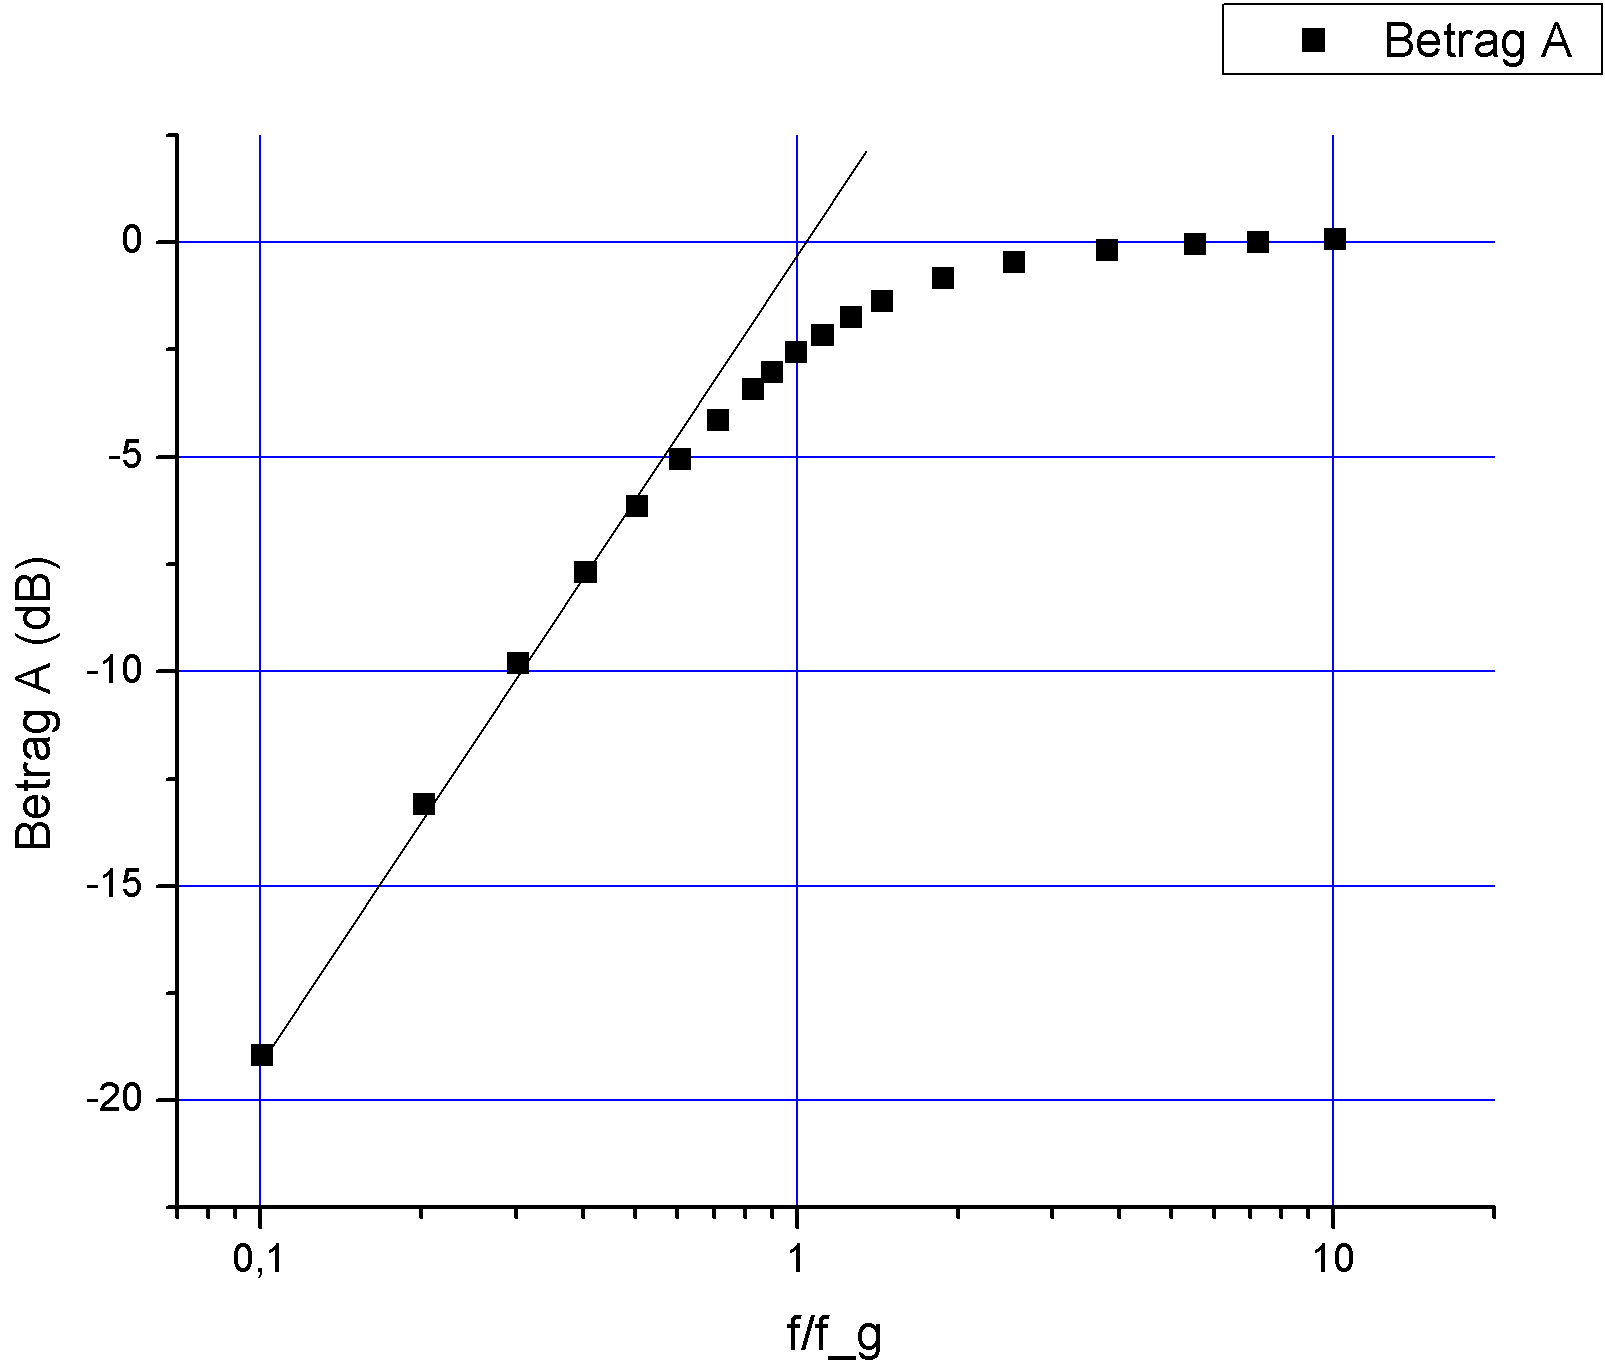
\includegraphics[scale=0.25]{./figure/betrag_a.png}
	\caption{Messung Betrag A mit linearem Fit}
	\label{fig:betraga_linfit}
\end{figure}
\begin{figure}[H]
	\centering
	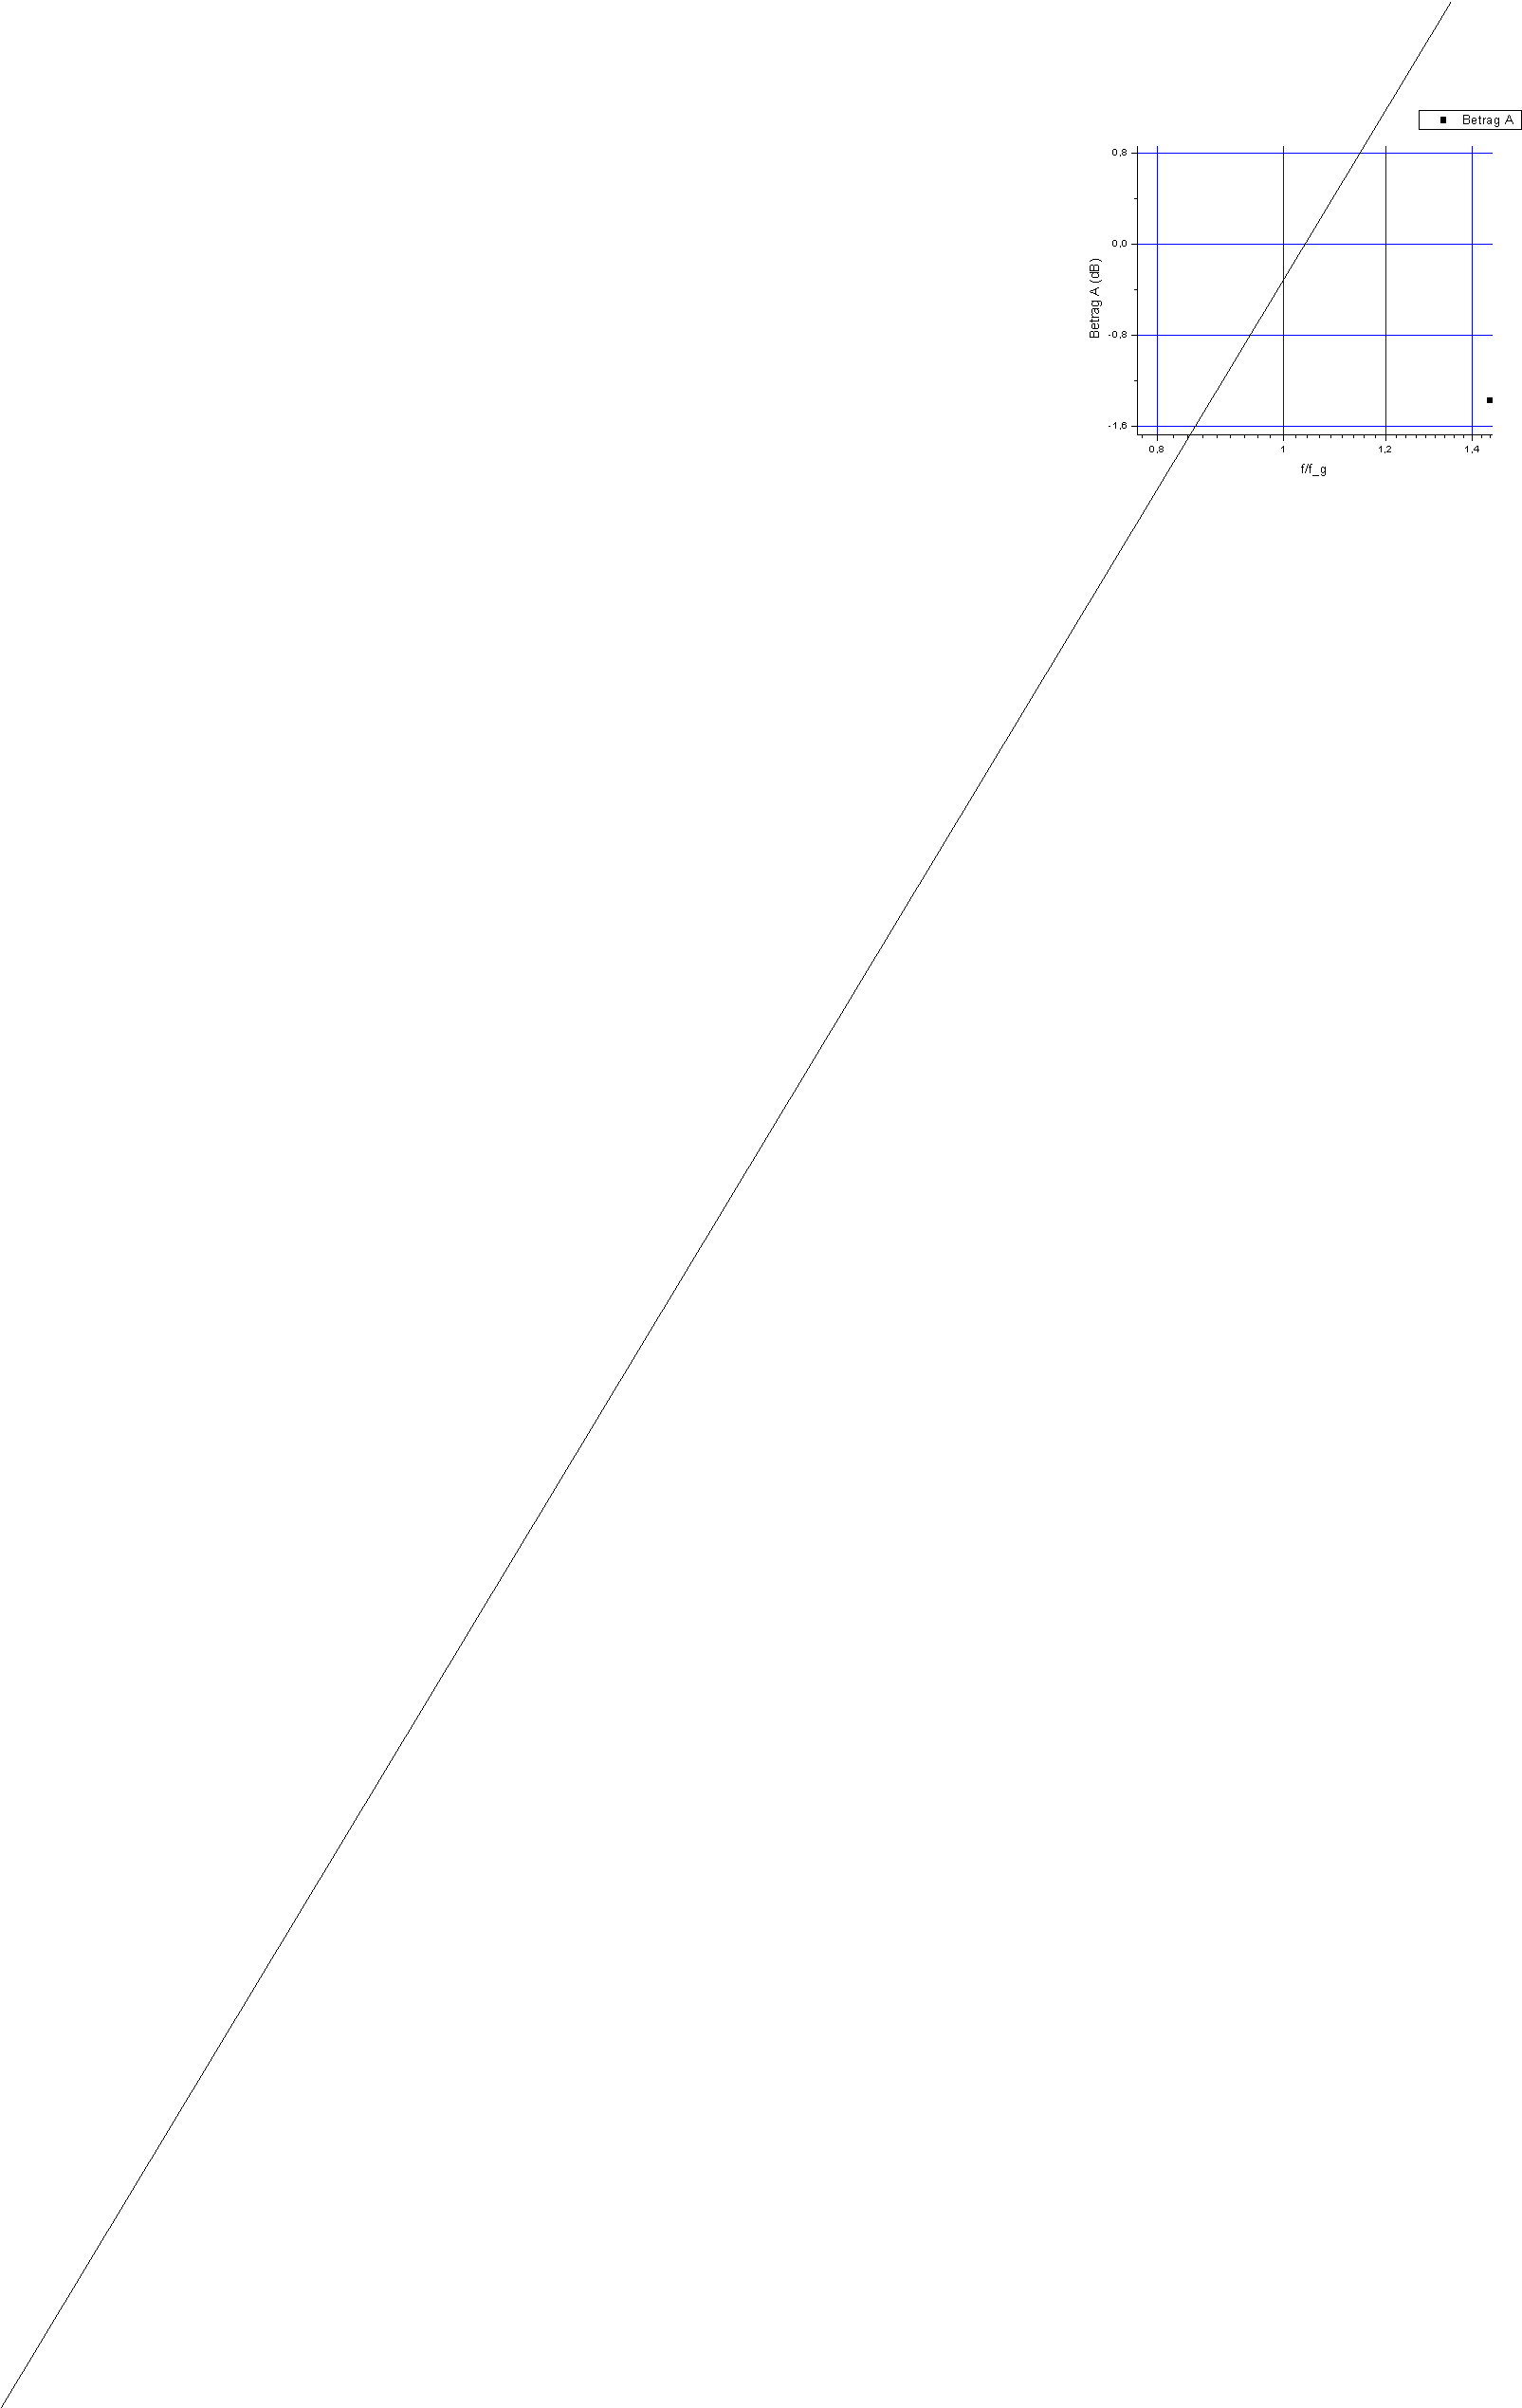
\includegraphics[scale=0.45]{./figure/betrag_a_zoom.png}
	\caption{Messung Betrag A Fehlerabschätzung}
	\label{fig:betraga_abweichung}
\end{figure}

\section{Diskussion}

%%%%%%%%%%%%%%%%%%%%%%%%%%%%%%%%%%%%%%%%%%%%%%%%


\section{Quellen}
$[1]$ Anleitung, \url{http://www.univie.ac.at/anfpra/neu1/pw/pw11/PW11.pdf}\\
\end{multicols}


\end{document}